\documentclass[journal,10pt]{IEEEtran}
\usepackage[T1]{fontenc}
\renewcommand{\ttdefault}{lmtt}
\usepackage{microtype,booktabs,tabularx,array,graphicx,xurl,amsmath}
\usepackage[hidelinks]{hyperref}
\hypersetup{pdftitle={When Does AI Beam Prediction Save Radio Resources? Cell-Level Accounting for AI-Native 6G},pdfauthor={Deepak Singh}}
\newcolumntype{Y}{>{\raggedright\arraybackslash}X}
\emergencystretch=1em
\raggedbottom
\title{When Does AI Beam Prediction Save Radio Resources? Cell-Level Accounting for AI-Native 6G}
\author{Deepak Singh\thanks{Deepak Singh is with the School of Computer Science, Kyungpook National University, Daegu, Republic of Korea (e-mail: deepak.singh@knu.ac.kr).}}
\begin{document}
\maketitle
\begin{abstract}
Monitoring timing can reverse which AI beam-management design saves more cell resources. We study 64-user ray-traced cells with full adoption of an error-free oracle. In New York, synchronized monitoring measurements (audits) of the sixteen highest-ranked beams every eighth update save 55.4 CSI-RS occurrences per update. Four-beam audits every second update save 39.3. Under independent uniform audit phases, mean expected savings become 12.5 and 21.8, reversing that ordering in all thirty cohorts despite unchanged per-UE budgets and intervals. The ordering also reverses in all thirty Los Angeles cohorts. In three of them, independently phased sixteen-beam audits raise expected load above the conventional baseline. We explain this result through three complementary accounts: UE observations, shared cell transmissions, and residual active time. Prediction releases cell resources when removable baseline demand exceeds additional input and monitoring demand, and supported controls realize that removal. The largest mean savings occur near full adoption with coordinated audits; the New York synchronized full-adoption examples release 0.110--0.155 percentage points of an illustrative time-frequency grid. Remaining consumers and resource placement determine the benefit at lower adoption and whether released transmissions create idle slots. The framework connects beam-quality qualification, monitoring schedules and existing resource-control mechanisms for 6G evaluation.
\end{abstract}

\section{When Fewer Measurements Release Radio Resources}
Two monitoring designs can spend the same average UE measurement budget yet reverse their ranking in cell-level resource savings simply because their monitoring measurements, called audits here, occur at different times. In our full-adoption examples from two cities, broader, less frequent audits save more transmissions when the UEs audit together. Independently phasing those same periodic audits makes the narrower design more economical in expectation. The predictor and each UE's measurement budget and audit interval are unchanged; the difference comes from sharing physical transmissions.

This gives a direct answer to the title question: AI beam prediction saves cell-level reference-signal resources when the baseline transmissions that can be removed outweigh the additional transmissions required for prediction inputs and monitoring, and resource controls can realize that removal. At a common beam-quality target, the strongest savings in our shared-bank study occur near full adoption with coordinated audits. More generally, the answer depends on who still needs each occurrence and when they need it.

Measurement-count metrics answer an earlier question. BM-Case1 in TR~38.843, Clause~6.3.1, compares input observations with the prediction domain, or total AI and baseline observations including additional measurements~\cite{tr38843}. A base station, however, transmits the union of compatible requests. A signal omitted by one user equipment (UE) may remain necessary for another UE, for prediction inputs, or for link supervision. In the mixed-cell example below, aggregate UE observations fall by 43.8\%, while CSI-RS occurrences fall by 1.7\%.

The Release-20 6G study item RP-251881 calls for AI/ML use cases with compelling performance and complexity tradeoffs and coordinated lifecycle management~\cite{sixgsid}. Xue et al. explain the beam-management standardization context~\cite{xue2024}, and Jayaweera et al. evaluate integrated prediction and monitoring~\cite{jayaweera2024}. Li et al. demonstrate time-domain beam prediction through over-the-air experiments~\cite{li2023}; Sun et al. study model selection and monitoring for beam management~\cite{sun2024}. We complement these predictor and lifecycle studies with the physical-transmission account needed to interpret a cell-level saving.

Figure~\ref{fig:architecture} follows three steps: count UE observations, reconcile shared transmissions, and inspect the residual active schedule. Beam quality constrains every step. We compare validation-selected conventional profiles with an error-free oracle requiring no fresh CSI-RS input. An exploratory New York study is followed by a Los Angeles check with the protocol fixed before its results. This optimistic reference case isolates the accounting mechanism; the same framework applies to learned predictors and conventional measurement-reduction methods once their inputs and monitoring demand are supplied.

\begin{figure*}[t]
\centering
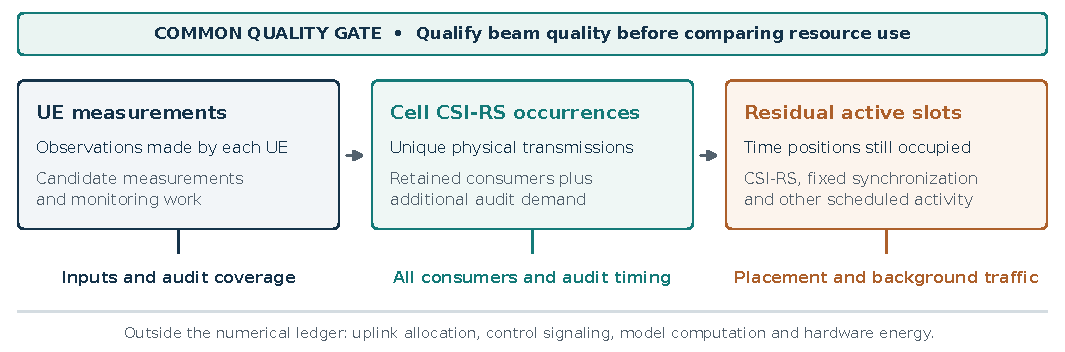
\includegraphics[width=\textwidth]{figures/accounting_architecture.pdf}
\caption{From receiver work to usable idle time. Quality qualification, retained consumers, audit timing and physical placement determine which savings can be claimed. The three accounts are complementary; a reduction in one does not establish the same reduction in the next.}
\label{fig:architecture}
\end{figure*}


\section{From Beam Prediction to Resource Control}
\subsection{Prediction and monitoring}
A synchronization signal block (SSB) supports cell discovery and synchronization. A channel-state-information reference signal (CSI-RS) is separately configurable and supports channel and beam measurements. Broad beam search is commonly described as P1; P2 refines the base-station transmit beam; P3 refines the UE receive beam while the transmit beam is fixed~\cite{jayaweera2024}.

The AI/ML study distinguishes spatial beam prediction (BM-Case1) from temporal prediction (BM-Case2). Set~A denotes the prediction domain; Set~B supplies observations and can differ from, or be a subset of, that domain~\cite{tr38843,jayaweera2024}. Prediction inputs belong in the resource account. Reusing an already retained SSB observation adds no CSI-RS input occurrence, whereas fresh CSI-RS observations must be charged.

Monitoring must also name its objective. Measuring predicted candidates can detect weak candidates; discovering a stronger unmeasured beam requires broader coverage. Jayaweera et al. describe Set-A monitoring~\cite{jayaweera2024}, while Sun et al. connect measured and predicted beam quality to model monitoring and selection~\cite{sun2024}. Audit coverage and interval therefore need to accompany any average measurement budget.

\subsection{The controller must release the signal}
Release-19 TS~38.300 describes prediction applicability, activation and performance monitoring~\cite{ts38300}. TS~38.214 distinguishes measurement and prediction resource settings and prediction reporting~\cite{ts38214}. RRC supplies resource and reporting configurations through TS~38.331~\cite{ts38331}, and TS~38.321 separates semipersistent resource-set activation from report control~\cite{ts38321}. Releasing a transmission consequently requires checking its resource configuration and all remaining consumers, including tracking, radio-link monitoring and beam-failure detection.

Resource limits depend on the configuration. In TS~38.214 V19.4.0, Clause~5.2.1.4.2, the restriction to at most sixteen resources in a set applies to the listed report quantities when the resource type is aperiodic and the linked setting is not configured for channel prediction~\cite{ts38214}. Our 64-beam bank represents a pool of physical occurrences across configurations. Control granularity matters too: if an activation command operates on an indivisible set, one required member can keep the entire set active. Reconfiguration, effective times and transition costs are part of realizing the accounting opportunity.

\section{Count the Transmissions That Can Disappear}\label{sec:contract}
A physical occurrence has a time, frequency, waveform and spatial transmission identity. Several UE-local resource identifiers can refer to one compatible occurrence. For example, two UEs configured to measure that same occurrence need only one transmission. If one stops measuring, the other can keep it active. Requests for different occasions or incompatible transmission parameters remain separate, even when their beam labels match.

For equal-sized occurrences and synchronized audits, the average transmitted CSI-RS count follows
\begin{equation}
N=R+qA.
\label{eq:accounting}
\end{equation}
Here $N$ is the average count per update, $R$ is the count retained every update, $A$ counts additional occurrences on an audit update, and $q$ is the audited fraction of updates. Retained demand includes conventional UEs, other consumers and fresh prediction inputs. Audits already covered by retained demand add UE work without adding transmissions. Unequal-sized occurrences require weighting by occupied resource elements (RE); different audit phases require averaging the joint schedule.

A saving occurs when the baseline count exceeds this post-activation count. For nonzero additional audit demand, the break-even synchronized duty is the baseline count minus the retained count, divided by the additional audit count. Fixed SSB cancels from the absolute difference but remains in a total reference-signal denominator.

The opposite sharing limit is instructive. If all UE-specific occasions are disjoint, equal-sized and separately removable, their costs add directly. With sixteen conventional observations and two average audit observations per AI UE, a 64-user baseline needs 1,024 occurrences; half adoption needs 576, and full adoption needs 128. The respective savings are 43.75\% and 87.5\%. Top-four and top-sixteen auditing then have equal average transmission cost, regardless of phase. This algebraic limiting case uses a different physical-occurrence baseline from the shared-bank experiment and isolates why sharing changes its result.

\begin{table*}[t]
\caption{Existing controls and the additional evidence needed for a resource decision. The additional records are proposed implementation or evaluation information.}
\label{tab:contract}
\small
\begin{tabularx}{\textwidth}{@{}>{\raggedright\arraybackslash}p{0.16\textwidth}>{\raggedright\arraybackslash}p{0.36\textwidth}Y@{}}
\toprule Responsible party & Existing mechanism or local source & Additional information needed for the decision \\\midrule
Model/profile supplier & Release-19 capability and applicability procedures; CSI-ReportConfig prediction and monitoring configuration~\cite{ts38300,ts38331}. & Quality population, required fresh observations, outputs and conditions requiring fallback. \\
Monitoring designer & Network-led performance monitoring in TS~38.300, Clause~22.2.4; configured measurement/report resources~\cite{ts38300,ts38331}. & Detectable failure, audit coverage, timing, detection-delay target and incremental physical demand. \\
gNB resource controller & RRC resource configuration plus implementation-local scheduler and consumer records~\cite{ts38331}. & Map UE-local identifiers to shared occurrences; check every consumer and residual activity before release. \\
Protocol implementer & Supported RRC reconfiguration, MAC resource-set activation/deactivation and applicable triggers~\cite{ts38331,ts38321}. & Capability checks, effective time, transition cost and confirmation that signals, not merely reports, change. \\
Operator & Quality/risk policy and implementation-specific supervisory control. & Choose the objective: UE work, occupied RE or usable idle time; require evidence for that objective. \\
\bottomrule
\end{tabularx}
\end{table*}

Table~\ref{tab:contract} links the evidence to existing controls. The gNB can maintain these records locally: qualify the profile, map all consumers to occurrences, charge the monitoring schedule, and apply supported changes. The proposed addition is a traceable evaluation record connecting those decisions. For 6G evaluation, report mixed-capability populations, UE observations, transmitted RE and absolute residual active time over a stated observation window.

\section{Qualify the Baseline Before Counting Savings}
We use DeepMIMO~\cite{deepmimo2019} and two public 28-GHz ray-traced scenarios: \texttt{city\_0\_newyork\_28} for the primary study and \texttt{city\_1\_losangeles\_28} for confirmation~\cite{citydata}. Each uses its first indexed base station, a modeled 64-element half-wavelength linear array and 64 DFT transmit beams. A single isotropic receiver confines the examples to transmit-beam refinement.

The bank is the cell's candidate resource pool: in the New York case, each conventional UE requests sixteen occurrences, and the cell transmits their union. A shared bank applies when several UEs measure the same physical CSI-RS occasions, for example compatible periodic or semipersistent resources with common timing, mapping, sequence and transmit beam~\cite{ts38214,ts38331}. Dedicated aperiodic triggers approach the disjoint limit when they schedule distinct occasions; aligned triggers for compatible resources can still share a transmission. Our illustrative refinement schedule isolates the shared regime; a deployment's resource map determines its position between these limits.

Conventional candidate profiles use previously measured full-bank rankings, contiguous neighborhoods around the previous best beam, or neighborhoods around separated high-power centers. They select from those lists using current noisy measurements. Prior and current measurement errors are independent, with 0.5-dB Gaussian errors and 1-dB quantization. Candidate lists are constructed entirely from prior information.

Before computing Los Angeles outcomes, we carried forward both quality rules from the New York protocol documented in the October~1 repository snapshot~\cite{projectrepo}. Among 22 profiles, validation selects the shortest measurement list whose 95\% geographic tile-bootstrap interval has a lower bound of at least 95\% success within 3~dB of the current best beam. On held-out locations, the selected profile must achieve a point estimate of at least 95\% success. We report its full evaluation interval. Figure~\ref{fig:quality} selects prior-top-16 (T16) for New York. It achieves 96.9\% validation success and 98.75\% evaluation success, with respective 95\% intervals of 95.7--98.0\% and 97.9--99.5\%. The 32-beam contiguous profile, C32, reaches 96.7\% on evaluation. Thus reusing prior rankings halves measurements while improving endpoint quality in this population.

\begin{figure}[t]
\centering
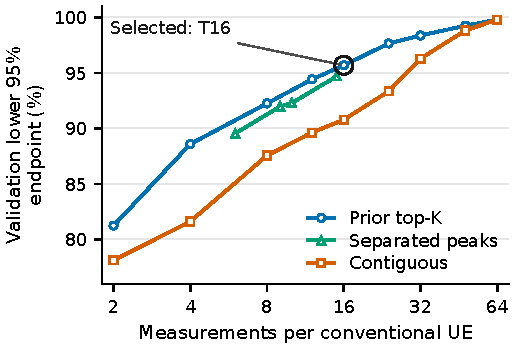
\includegraphics[width=\columnwidth]{figures/quality_qualified.pdf}
\caption{New York validation selects prior-top-16 (T16) as the lowest-measurement qualifier among the tested profiles. The vertical quantity is the lower endpoint of a geographic tile-bootstrap 95\% interval; the quality threshold is 95\% success within 3~dB.}
\label{fig:quality}
\end{figure}


New York evaluation covers 8,884 directional pairs over 2,469 current locations and seventeen geographic tiles. The oracle reaches the true best beam; both arms meet the same minimum quality requirement. The companion package documents the profile list, tie rules, spatial pairing and resampling details~\cite{projectrepo}.

Los Angeles was selected as the next numbered distinct city in the same 28-GHz scenario family before computing its results. We retain the array, one-metre pairing, 20-m geographic tiles with 2-m boundary guards, noise seeds, candidate families and selection rule. Validation selects two separated three-beam neighborhoods (L2x3, six measurements): success is 97.09\% with a 95\% interval of 95.17--98.57\%. Evaluation gives 95.88\% [92.88--98.00\%] over 9,102 pairs, 2,496 current locations and fourteen tiles. The point estimate meets the prespecified evaluation threshold. The interval also includes success rates below 95\%.

The primary unit is one refinement after a 1-m displacement between sampled locations. For time-frequency conversion, an illustrative 80-ms window corresponds to 1~m at 45~km/h. The separate 20-ms SSB period contributes four bursts in that window. The unchanged New York T16 profile reaches 97.4\% success at 2~m and 93.8\% at 5~m, illustrating its operating envelope.

Both arms condition on an available prior full-bank measurement, whose common initialization cost is excluded from the recurring counts. In New York, a refresh sensitivity replaces every tenth conventional update with a synchronized full sweep: mean cell occurrences change from 63.27 to 63.34, while UE observations rise from 1,024 to 1,331, about 30\%. The shared bank makes refresh inexpensive at cell level even when it substantially increases receiver work. Refresh in the mixed arm can also reduce partial-adoption savings.

\section{Audit Coordination Changes the Preferred Design}\label{sec:monitoring}
For each New York population size, we use thirty cohorts of distinct current locations, one eligible prior location per UE, and nested random AI adoption independent of channel quality. All monitoring designs share the same cohorts and assignments. Conventional UEs use T16; oracle-served UEs use the true best beam, with ideal current rankings also defining audit lists.

Three New York designs spend two average observations per AI UE per update: the four highest-ranked beams (top-four) every second update, the sixteen highest-ranked beams (top-sixteen) every eighth update, and four geometric neighbors around the ideal best beam every second update. In the time illustration, the first and third audit every 160~ms, and the broader design audits every 640~ms. These budgets support different coverage and detection intervals.

\subsection{The ranking reverses when phases change}
At full adoption in the 64-user New York cell, synchronized top-four audits save 39.3 occurrences per update; synchronized top-sixteen audits save 55.4. The broader design benefits because many UEs' audit requests can be served together on an infrequent common update.

To isolate that coordination effect, we use the same saved cohorts and fixed endpoint demands. Each UE still audits once every two or eight updates, but independently selects a uniform phase within that period. We calculate the exact expected occupancy over phase assignments, preserving each UE's budget and interval.

Consider one occurrence that only audits require. Suppose it appears on the fixed lists of $k\geq 1$ UEs, each auditing once every $P$ updates. With synchronized phases, all requests fall on one update per period. With independent uniform phases, the occurrence is needed whenever at least one UE is due. The corresponding expected fractions of updates occupied are
\begin{equation}
  p_{\mathrm{sync}}=\frac{1}{P}, \qquad
  p_{\mathrm{ind}}=1-\left(1-\frac{1}{P}\right)^{k}.
  \label{eq:auditphase}
\end{equation}
For two UEs auditing every second update, these fractions are one half and three quarters. With a single requester the timing penalty vanishes. As more UEs share an occurrence at a fixed period, independent phases push its occupancy toward one. An occurrence already required on every update by a conventional UE adds zero audit transmissions under either schedule.

At full adoption in New York, summing (\ref{eq:auditphase}) over the requested occurrences gives the mean occupancy per update out of 64 possible occurrences. With synchronized audits, top-four occupies 24.00 and top-sixteen 7.89. With independent phases, top-four occupies 41.50 and top-sixteen 50.78 in expectation. The ordering reverses in all thirty cohorts (Table~\ref{tab:phase}). The synchronized advantage of top-sixteen ranges from 13.5 to 18.9 occurrences per update across cohorts; the independent-phase advantage of top-four ranges from 6.4 to 13.8. Figure~\ref{fig:budget} shows both timing modes and their cohort spread. Audit-phase coordination is therefore part of the resource claim; the calculation holds demands fixed over its accounting period.

\begin{table}[t]
\caption{Mean CSI-RS occurrences saved per update under synchronized and independently phased periodic audits. Each scene uses 30 fixed 64-user cohorts and its validation-selected conventional baseline. A third decimal shows the small timing differences at half adoption.}
\label{tab:phase}
\centering\small
\begin{tabular}{@{}llrr@{}}
\toprule Adoption & Audit / period & Synchronized & Independent \\\midrule
\multicolumn{4}{l}{New York: T16 baseline (16 measurements)} \\
50\% & Top-4 / 2 updates & 1.083 & 1.075 \\
50\% & Top-16 / 8 updates & 0.967 & 0.847 \\
100\% & Top-4 / 2 updates & 39.27 & 21.77 \\
100\% & Top-16 / 8 updates & 55.38 & 12.49 \\\midrule
\multicolumn{4}{l}{Los Angeles: L2x3 baseline (6 measurements)} \\
100\% & Top-4 / 2 updates & 30.90 & 17.57 \\
100\% & Top-16 / 8 updates & 44.75 & 5.25 \\\bottomrule
\end{tabular}
\end{table}

\subsection{Remaining users determine partial-adoption savings}
New York conventional demand occupies an average of 63.27 of the 64 available occurrences in the 64-user cell. At half adoption, the remaining users still require 62.17. Synchronized top-four auditing then saves 1.083 occurrences per update, or 1.71\%, while UE observations fall from 1,024 to 576, or 43.75\%. The retained demand leaves little room for audit timing to change cell occupancy. Top-four yields the larger mean saving under both schedules at half adoption (Table~\ref{tab:phase}).

\begin{figure}[t]
\centering
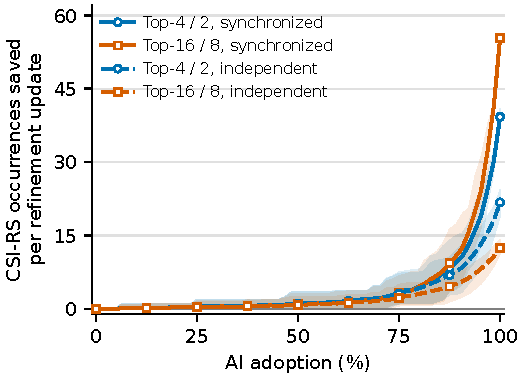
\includegraphics[width=\columnwidth]{figures/equal_budget.pdf}
\caption{Mean CSI-RS occurrences saved per update in the 64-user New York cell. Solid lines: synchronized audits; dashed: exact independent-phase expectations. Bands show cohort 5th--95th percentiles, not confidence intervals. Legend periods are in updates; each design averages two observations per AI UE. Curves use every integer adoption count in the same 30 cohorts.}
\label{fig:budget}
\end{figure}


The effect depends on demand concentration and population. At half adoption, top-four audits save 5.42 occurrences with sixteen users, 2.97 with thirty-two, and 1.08 with sixty-four. Independent uniform sixteen-beam lists would release only about 0.0064 occurrences when the conventional population falls from sixty-four to thirty-two, before audits; this site's observed decrement is 1.10. Explicit user placement and beam demand therefore matter when estimating the retained-resource floor.

The top-four versus top-sixteen half-adoption difference is small: the paired mean is 0.117 occurrences, with a cohort range from a 0.375-occurrence loss to a 0.750-occurrence gain. A separate duty sweep gives a mean-count break-even duty of 0.877 for top-sixteen audits at half adoption with thirty-two users. Such a threshold identifies the occupancy balance; the monitoring designer must separately choose an acceptable detection interval.

\subsection{A second city preserves the reversal}
The frozen Los Angeles check repeats the top-four and top-sixteen schedules on thirty 64-user cohorts. Its six-measurement baseline occupies a mean of 52.7 shared occurrences. At full adoption, Table~\ref{tab:phase} shows synchronized mean savings of 30.90 and 44.75, versus independent-phase expected savings of 17.57 and 5.25. The expected ordering reverses in all thirty cohorts: the synchronized top-sixteen advantage ranges from 10.5 to 17.5, and the independent-phase top-four advantage from 9.3 to 15.6. At full adoption the two designs share the same baseline, so subtracting their savings leaves only the difference in audit occupancy. The baseline sets the absolute saving. In three cohorts, independent top-sixteen auditing increases expected demand by up to 4.44 occurrences per update. Coordination and baseline efficiency both matter when converting a monitoring budget into a resource claim.

\subsection{Report the absolute scale}
For the New York example, the illustrative grid contains 640 slots over 80~ms, 48 resource blocks, fourteen symbols per slot and 120-kHz subcarrier spacing: about 5.16 million RE. Four bursts of eight SSBs occupy 26,560 nonzero RE. A row-1 one-port CSI-RS with density three occupies 144 RE over those resource blocks~\cite{ts38211}. This ledger counts nonzero signal elements; scheduler reservations and usable payload capacity require their own mapping.

At half adoption, the 1.71\% CSI-RS occurrence saving occupies just 0.0030 percentage points of the grid. At full adoption with synchronized audits, top-four and top-sixteen save 62.1\% and 87.5\% of CSI-RS occurrences, 15.9\% and 22.4\% of the SSB-plus-CSI-RS footprint, and 0.110 and 0.155 percentage points of the grid. The rounded 87.5\% matches the disjoint-limit percentage, but uses a different baseline: about 63.27 shared occurrences rather than 1,024 dedicated occurrences. These denominators distinguish a large relative CSI-RS reduction from a small absolute grid saving.

For top-sixteen auditing, reducing the common SSB schedule from four bursts to one increases the RS-footprint saving from 22.4\% to 50.6\%, while the absolute saving remains 7,975 RE. Using row-2 density-one CSI-RS instead reduces the same request saving to 2,658 RE, or 0.0515 percentage points of the grid~\cite{ts38211}. These fixed-demand sensitivities illustrate how signal density changes the resource account; changed measurement quality and input cadence require separate qualification. The on-demand SSB procedure described in Release~19 has a secondary-cell carrier-aggregation scope~\cite{ts38300}.

\section{Resource Placement Determines Idle Time}
An RE saving creates idle time when the removed transmissions are the last activity in the relevant symbols or slots. Cell DTX/DRX motivates evaluating this residual activity~\cite{ts38300}.

For the 64-user New York cell with synchronized top-four audits, we compare two fixed mappings used identically in both arms. The sparse map assigns two successive beam indices per slot, on symbols four and eight, beginning at slot four. The packed map places fourteen successive indices per slot, one per symbol, from the same starting slot. The complete bank spans thirty-two or five slots. SSB retains its Case-D positions and 20-ms cadence~\cite{ts38213}. Independent background activity is absent, present in every fourth slot, or continuous.

At half adoption with top-four monitoring, both mappings release a net mean of 1.08 active symbols. Sparse placement releases 0.167 slots; packed placement releases zero because residual CSI-RS touches all five slots. At full adoption without independent traffic, Figure~\ref{fig:packing} shows the absolute CSI-bearing slot counts: about 31.9 to 13.1 for sparse placement and five to 2.05 for packed placement. Fixed SSB adds sixteen unchanged active slots.

\begin{figure}[t]
\centering
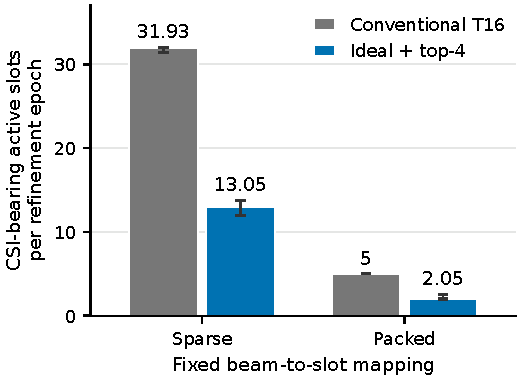
\includegraphics[width=\columnwidth]{figures/packing_comparison.pdf}
\caption{Absolute CSI-bearing active slots at full adoption with synchronized top-four auditing every second update, for 64 New York users. Whiskers are cohort 5th--95th percentiles. Fixed SSB adds sixteen unchanged active slots.}
\label{fig:packing}
\end{figure}


Packing starts and finishes with fewer active slots, although its reduction is smaller. With every fourth slot independently active, net reductions become 13.9 slots for sparse placement and 1.50 for packed placement; continuous activity makes both zero. Report the final active schedule alongside the reduction. Translating idle opportunities into energy additionally requires minimum sleep duration, wake-up cost, traffic deadlines and hardware behavior.

\section{Deployment Implications and Study Limits}
An operator can apply the framework by qualifying beam quality, reconciling all physical consumers, evaluating the actual audit schedule, and checking supported resource-control actions. A profile merits activation for an occupancy objective when these steps yield positive net removal. An idle-time objective additionally requires examining where residual traffic remains. The decision record can initially reside inside the gNB; transporting it across vendors is a separate interface question.

The evidence covers two simulated sites from the same ray-tracing family, one base station per site, one channel-frequency sample, one receive antenna, and thirty cohorts per evaluated population. In the exploratory New York study, profile families were extended after earlier contiguous-baseline results were inspected; the added selection rule was fixed before the reported outcomes were computed. Its phase comparison was added after inspecting synchronized results. The Los Angeles protocol was fixed before computing that scene's outcomes; its selected baseline's evaluation interval crosses the 95\% quality target despite passing the point-estimate gate. The 3-dB proxy is distinct from standardized wideband RSRP over the accounting allocation. An error-free oracle and ideal audit rankings favor prediction, while prior-refresh omissions affect the two arms differently; the result is an optimistic reference case, not a universal upper bound. Both phase analyses hold endpoint demands fixed, and placement assumes ideal beam switching. Sustained mobile tracking, detection and recovery performance, resource-set realizability, control transactions, uplink allocation and model computation require additional evaluation.

Deployment validation still requires a learned predictor with charged inputs and fallback, and a time-consistent comparison at matched beam-quality and detection targets. The companion package contains analysis code, source provenance, prepared second-scene inputs, saved results and supplementary methods; its repository landing page is~\cite{projectrepo}.

\section{Conclusion}
AI beam prediction saves cell-level reference-signal resources when removable baseline transmissions exceed incremental input and monitoring demand, and supported controls can realize the change. The largest mean opportunities occur near full adoption with coordinated audits; the New York synchronized full-adoption savings occupy 0.110--0.155 percentage points of the illustrative grid. Independent audit phases reverse the expected ordering of the two monitoring designs in all thirty full-adoption cohorts of each city. Mean savings remain positive, while some Los Angeles cohorts incur extra demand under broader independent audits. Remaining consumers govern partial-adoption gains, and physical placement governs idle time. Report these conditions with predictor quality so that a reduction in UE measurements can be translated into a defensible cell-level claim.

\section*{Acknowledgment}
ChatGPT (OpenAI) assisted with drafting and revising the article, source checking, analysis and plotting code, and figure preparation. The companion package records earlier computational reruns and reconstruction checks performed with this assistance. For this revision, ChatGPT also assisted with the exact audit-phase calculations, the second-scene execution and independent numerical checks, and presentation checks.

\begin{thebibliography}{15}
\bibitem{tr38843}
3GPP, {\em Study on Artificial Intelligence ({AI})/Machine Learning ({ML}) for
  {NR} Air Interface}, Sept. 2025.
\newblock TR 38.843, V19.0.0. Clause 6.3.1. [Online]. Available: \url{https://www.3gpp.org/ftp/Specs/archive/38_series/38.843/38843-j00.zip}. Accessed on: Oct. 5, 2026.

\bibitem{sixgsid}
3GPP, ``New SID: Study on 6G Radio,'' RP-251881, TSG RAN\#108, June 2025. [Online]. Available: \url{https://www.3gpp.org/ftp/tsg_ran/TSG_RAN/TSGR_108/Docs/RP-251881.zip}. Accessed on: Oct. 5, 2026.

\bibitem{xue2024}
Q.~Xue, J.~Guo, B.~Zhou, Y.~Xu, Z.~Li, and S.~Ma, ``{AI/ML} for beam management
  in {5G-Advanced}: A standardization perspective,'' {\em IEEE Vehicular
  Technology Magazine}, vol.~19, no.~4, pp.~64--72, 2024.
\newblock doi:
  10.1109/MVT.2024.3431790. Author manuscript: \url{https://arxiv.org/abs/2309.10575}. Accessed on: Nov. 16, 2026.

\bibitem{jayaweera2024}
N.~Jayaweera, A.~Bonfante, M.~Schamberger, A.~M.~A. Tehrani, T.~Sanguanpuak,
  P.~Tilak, K.~Jayasinghe, F.~W. Vook, and N.~Rajatheva, ``{5G-Advanced AI/ML}
  beam management: Performance evaluation with integrated {ML} models.''
  arXiv:2404.15326v1, 2024.
\newblock \url{https://arxiv.org/html/2404.15326v1}. Accessed on: Nov. 16, 2026.

\bibitem{li2023}
Q.~Li et al., ``Machine learning based time domain millimeter-wave beam prediction for 5G-Advanced and beyond: Design, analysis, and over-the-air experiments,'' {\em IEEE Journal on Selected Areas in Communications}, vol.~41, no.~6, pp.~1787--1809, June 2023. doi:~10.1109/JSAC.2023.3275613. [Online]. Available: \url{https://doi.org/10.1109/JSAC.2023.3275613}. Accessed on: Nov. 17, 2026.

\bibitem{sun2024}
C.~Sun, L.~Zhao, T.~Cui, H.~Li, Y.~Bai, S.~Wu, and Q.~Tong, ``AI model selection and monitoring for beam management in 5G-Advanced,'' {\em IEEE Open Journal of the Communications Society}, vol.~5, pp.~38--50, 2024. doi:~10.1109/OJCOMS.2023.3337850. [Online]. Available: \url{https://doi.org/10.1109/OJCOMS.2023.3337850}. Accessed on: Nov. 17, 2026.

\bibitem{ts38300}
3GPP, {\em {NR; NR and NG-RAN} Overall Description; Stage 2}, Aug. 2026.
\newblock TS 38.300, V19.3.0.
  \href{https://www.etsi.org/deliver/etsi_ts/138300_138399/138300/19.03.00_60/ts_138300v190300p.pdf}{Official
  ETSI edition}. Accessed on: Nov. 16, 2026.

\bibitem{ts38214}
3GPP, {\em {NR}; Physical Layer Procedures for Data}, July 2026.
\newblock TS 38.214, V19.4.0.
  \href{https://www.etsi.org/deliver/etsi_ts/138200_138299/138214/19.04.00_60/ts_138214v190400p.pdf}{Official
  ETSI edition}. Accessed on: Nov. 16, 2026.

\bibitem{ts38331}
3GPP, {\em {NR}; Radio Resource Control ({RRC}); Protocol Specification}, Aug.
  2026.
\newblock TS 38.331, V19.3.0.
  \href{https://www.etsi.org/deliver/etsi_ts/138300_138399/138331/19.03.00_60/ts_138331v190300p.pdf}{Official
  ETSI edition}. Accessed on: Oct. 5, 2026.

\bibitem{ts38321}
3GPP, {\em {NR}; Medium Access Control ({MAC}); Protocol Specification}, Aug.
  2026.
\newblock TS 38.321, V19.3.0.
  \href{https://www.etsi.org/deliver/etsi_ts/138300_138399/138321/19.03.00_60/ts_138321v190300p.pdf}{Official
  ETSI edition}. Accessed on: Nov. 16, 2026.

\bibitem{deepmimo2019}
A.~Alkhateeb, ``{DeepMIMO}: A generic deep learning dataset for millimeter wave
  and massive {MIMO} applications.'' arXiv:1902.06435, 2019.
\newblock \url{https://arxiv.org/abs/1902.06435}. Accessed on: Oct. 5, 2026.

\bibitem{citydata}
{DeepMIMO}, ``{city\_0\_newyork\_28} and {city\_1\_losangeles\_28} scenarios.'' DeepMIMO scenario database; ray tracing with Remcom Wireless InSite. [Online]. Available: \url{https://www.deepmimo.net/scenarios/v4/city_0_newyork_28} and \url{https://www.deepmimo.net/scenarios/v4/city_1_losangeles_28}. Accessed on: Nov. 17, 2026.

\bibitem{projectrepo}
D. Singh, ``AI beam resource accounting: project repository,'' GitHub, 2026. [Online]. Available: \url{https://github.com/deepakkolhua/ai-beam-resource-accounting}. \href{https://github.com/deepakkolhua/ai-beam-resource-accounting/blob/cf37b694731835e08de04303e0457376e6d0c685/SNAPSHOT_README.md\#L39}{October 1 protocol snapshot}. Accessed on: Nov. 18, 2026.

\bibitem{ts38211}
3GPP, {\em {NR}; Physical Channels and Modulation}, July 2026.
\newblock TS 38.211, V19.4.0.
  \href{https://www.etsi.org/deliver/etsi_ts/138200_138299/138211/19.04.00_60/ts_138211v190400p.pdf}{Official
  ETSI edition}. Accessed on: Oct. 5, 2026.

\bibitem{ts38213}
3GPP, {\em {NR}; Physical Layer Procedures for Control}, July 2026.
\newblock TS 38.213, V19.4.0.
  \href{https://www.etsi.org/deliver/etsi_ts/138200_138299/138213/19.04.00_60/ts_138213v190400p.pdf}{Official
  ETSI edition}. Accessed on: Oct. 5, 2026.

\end{thebibliography}


\begin{IEEEbiographynophoto}{Deepak Singh}
(deepak.singh@knu.ac.kr) is with the School of Computer Science, Kyungpook National University, Daegu, Republic of Korea. His research interests include AI-native radio access networks, beam management and resource-efficient wireless communications.
\end{IEEEbiographynophoto}
\end{document}